\newpage

\chapter{Разработанное ПО}

\subsection{Требования к ПО}
Программное обеспечение разрабатывалось в учебных целях для исследования работы эволюционных алгоритмов в нейронных сетях и тестирования его эффективности.

\subsection{Выбор средств для создания ПО}

Для написания программы использовался язык программирования Python в связке со средой разработки Jupyter Notebook. Этот язык был выбран для написания выпускной работы бакалавра в связи с большим количеством библиотек, в которых реализованы основные методы для работы с матрицами, строками и файлами.
Среда разработки Jupyter Notebook позволяет удобно работать с кодом, подсвечивая синтаксис языка. Главной интересной функцией среды разработки является возможность компилировать код построчно, что позволяет увидеть ошибку сразу. 

\subsection{Описание созданного ПО}

Нужно научиться решать такую задачу:
Зная начальное направление (угол от поверхности земли) и скорость мяча, определить, где этот мяч упадёт. Или иначе: попадёт ли мяч в мишень, находящуюся на земле, при заданных начальных условиях.

\begin{figure}[h]
  \centering
  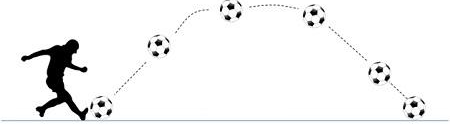
\includegraphics[width=0.5\linewidth]{./img/footbal}
  \caption{Удар по мячу}
  \label{fig:mpr} 
\end{figure} 

В данных у нас скорость удара, угол удара(угол между направлением полёта мяча и землёй) и расстояние до мишени. Скорость броска от 0 и до 50. Угол принимает значения из промежутка от 0 до $\frac{\pi}{2}$. 

Загружаем файл с данными.

\begin{lstlisting}
  data = np.loadtxt("data.csv", delimiter=",")
\end{lstlisting}

Разница в масштабах настолько существенна, что имеет смысл нормализовать наши данные, чтобы при обучении не отвлекаться на попытки скомпенсировать масштаб данных масштабом весов.

\begin{lstlisting}
  means = data.mean(axis=0)
  means[-1] = 0 
  stds = data.std(axis=0)
  stds[-1] = 1
  data = (data - means) / stds
\end{lstlisting}

Чтобы была возможность следить за успешностью обучения, сразу отделим часть данных в тестовое множество.

\begin{lstlisting}
  np.random.seed(42)
  test_index = np.random.choice([True, False], len(data), replace=True, p=[0.25, 0.75])
  test  = data[test_index]
  train = data[np.logical_not(test_index)]
\end{lstlisting}

Приведем  данные в тот вид, в котором они понимаются нейросетью. Для обучения нам нужно, чтобы ответ был в формате one-hot: вектор длины 3 (общее количество классов), состоящий из нулей и одной единицы на месте правильного класса наблюдения. Мы сделаем это с помощью np.eye: для единицы, стоящей на i-м месте, нужно создать вектор np.eye(3, 1, k=-i). Соответственно, когда мы будем итерироваться по нашим входным данным, искомое i для примера - это последний элемент строки с этим примером, то есть d(-1). 

\begin{lstlisting}
train = [(d[:3][:, np.newaxis], np.eye(3, 1, k=-int(d[-1]))) for d in train]  
test =  [(d[:3][:, np.newaxis], d[-1]) for d in test]
\end{lstlisting}

Зададим параметры нейронной сети:
\begin{itemize}
  \item inputCount - количество нейронов входного слоя
  \item hiddenCount - количество нейронов скрытого слоя
  \item outputCount - количество нейронов выходного слоя
  \item SIZE - размер популяции нейронных сетей
\end{itemize}

\begin{lstlisting}
  input_count  = 3 
  hidden_count = 7 
  output_count = 3   
  SIZE = 10 
\end{lstlisting}

Следующим этапом будет создание популяции из 10 особей нейронных сетей и применение эволюционного алгоритма к этой популяции.

Эволюционный алгоритм:
\begin{itemize}
  \item Создаем популяцию из 10 нейронных сетей с рандомными весами
  \item Обучаем каждую особь из популяции на тренировочной выборке и смотрим какой процент правильных ответов она выдает
  \item Выбираем 5 лучших особей по проценту правильных ответов
  \item Скрещиваем 2 самые лучшие особи и 4 пары из 5 лучших (получается 10 новых нейронных сетей)
  \item Проделываем пункты 2-4 пока по количеству эпох, в нашем случае будет 100 эпох (поколений нейросетей)
\end{itemize}

\begin{lstlisting}
  nn = []

for i in range(SIZE):
  network = Network([input_count, hidden_count, output_count]) percent =
  network.SGD(training_data=train, epochs=1, mini_batch_size=5,
  eta=1, test_data=test)
  nn.append((network, percent))

for epoch in range(100):
  nn.sort(key=lambda x: x[1])
  nn = nn[5:] 
  nnChild = []
  indexes = np.random.randint(0, 5, 10)
  np.random.shuffle(indexes) 
 
  nn[indexes[4]][0].genetic(nn[indexes[3]][0], nnChild) 

  for x in range(4):
    nn[indexes[x]][0].genetic(nn[indexes[x + 5]][0], nnChild)
  nn = nnChild
\end{lstlisting}

Каждая наша нейронная сеть имеет 3 слоя – входной, скрытый и выходной. Это означает, что веса нейронной сети будут храниться в 2-х массивах:

\begin{itemize}
  \item Первый массив – веса между входным и скрытым слоем, размерности $7\times3$
  \item Второй массив – веса между скрытым и выходным слоем, размерности $3\times7$
\end{itemize}

Алгоритм скрещивания работает следующим образом:

\begin{itemize}
  \item На вход подается 2 особи (нейронных сети)
  \item Выбираем случайным образом индекс из матрицы весов
  \item Создаем 2 новых потомка, таких, что в первом потомке будут веса из первой нейронной сети до номера случайного индекса, остальная часть из матрицы весов второй нейронной сети, а у второго потомка наоборот
  \item Обучаем алгоритмом обратного распространения ошибки и смотрим результат на тестовой выборке
  \item Возвращаем 2 новых нейронных сети с их результатами
\end{itemize}

После обучения выбираем нейронную сеть с самым лучшим результатом – это и будет итоговая сеть, которую можно использовать для решения реальных задач.

\subsection{Результаты тестирования ПО}

В ходе работы программы были выведены результаты обучения нейронной сети с использованием эволюционного алгоритма. Нейронная сеть обучалась на тренировочной выборке 100 раз. Ниже представлены результаты начальной эпохи, 51-й эпохи и последней эпохи.

В начале первое поколение нейронных сетей дает следующий результат. Как можно заметить, после первого обучения нейронные сети дают в среднем 40\% правильных ответов.

\begin{figure}[H]
  \centering
  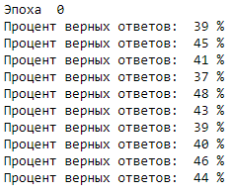
\includegraphics[width=0.4\linewidth]{./img/first-epoch}
  \caption{Начальное поколение нейронных сетей}
  \label{fig:mpr} 
\end{figure}

Поколение с номером 51 дает уже 73\% правильных ответов. Заметен существенный прирост в количестве верных ответов.

\begin{figure}[H]
  \centering
  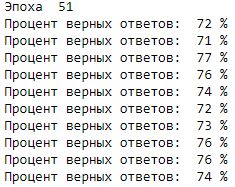
\includegraphics[width=0.4\linewidth]{./img/second-epoch}
  \caption{51 поколение нейронных сетей}
  \label{fig:mpr} 
\end{figure}

Последнее поколение будет отвечать на поставленную задачу правильно в 87\% случаев.

\begin{figure}[H]
  \centering
  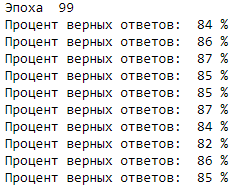
\includegraphics[width=0.4\linewidth]{./img/third-epoch}
  \caption{51 поколение нейронных сетей}
  \label{fig:mpr} 
\end{figure}

После прохождения 100 эпох получилась рабочая нейронная сеть, способная отвечать правильно на поставленную задачу в 87\% случаях. 